\documentclass[12pt]{article}
\usepackage{sbc-template}
\usepackage{graphicx,url,booktabs,array}
\usepackage[utf8]{inputenc}
\usepackage[T1]{fontenc}
\usepackage[brazil]{babel}
\usepackage{float}
\usepackage{microtype}
\sloppy

\title{Apoio à Triagem de Radiografias de Tórax com ResNet-50: Avaliação de Robustez e Grad-CAM}
\author{Alana Luize Kunrath\inst{1}, Murilo Ghedin Ghizzi\inst{1},\\
Mauro Junior Cella Schuastz\inst{1}, Lucas Henrique Bonissoni\inst{1},\\
Matheus de Aquino da Silva\inst{1}, Luiz Augusto Cenci\inst{1}}
\address{Universidade Tecnológica Federal do Paraná -- Campus Dois Vizinhos\\
Bacharelado em Engenharia de Software}
\begin{document}
\maketitle
\begin{abstract}
This paper studies a binary chest radiograph classifier for triage support. A ResNet-50 trained on a patient-separated subset of NIH ChestX-ray14 reached 0.904 recall and 0.679 F1 on 1,144 test images. We compared 150 original radiographs with five types of synthetic degradation. Balanced accuracy decreased from 0.600 to 0.520, while recall increased. Grad-CAM inspection of 15 cases found strong activation outside the lung fields in the three selected false negatives. The system is an academic prototype and requires external validation.
\end{abstract}
\begin{resumo}
Este artigo avalia um classificador binário de radiografias de tórax como apoio à triagem. Uma ResNet-50 treinada em uma amostra do NIH ChestX-ray14, com divisão por paciente, obteve recall de 0,904 e F1 de 0,678 em 1.144 imagens de teste. Comparam-se 150 radiografias originais com cinco degradações sintéticas. A balanced accuracy caiu de 0,600 para 0,520, embora o recall tenha aumentado. Na inspeção de 15 mapas Grad-CAM, os três falsos negativos selecionados tiveram ativação predominante fora dos pulmões. O sistema é um protótipo acadêmico que requer validação externa.
\end{resumo}

\section{Introdução}
O volume de radiografias de tórax pode exigir uma ordem de leitura que dê atenção antecipada aos exames com maior probabilidade de alteração. Este trabalho investiga um classificador de duas classes, NORMAL e ALTERADA, que atribui uma probabilidade de alteração e a converte em uma prioridade de fila. A saída apoia a organização da análise por profissionais, sem estabelecer diagnóstico ou substituir a leitura radiológica. O objetivo é medir sensibilidade, erros e robustez do sistema em dados públicos e em imagens degradadas sinteticamente. O código, os splits e os resultados estão em \url{https://github.com/LuizCenci/triagem-raio-x}.

\section{Dados}
O NIH Clinical Center disponibiliza o ChestX-ray14, com 112.120 radiografias frontais de 30.805 pacientes e rótulos extraídos de laudos \cite{wang2017chestxray}. Utilizou-se a amostra pública \url{https://www.kaggle.com/datasets/nih-chest-xrays/sample}, com 5.606 imagens identificadas nos splits versionados. A classe NORMAL corresponde a \textit{No Finding}; qualquer outro achado compõe ALTERADA. Os pacientes foram separados em treino (3.931 imagens), validação (531) e teste (1.144), sem interseção entre grupos. A avaliação final usa o teste isolado; a validação orienta limiares e limites de qualidade.

A origem das imagens é \url{https://nihcc.app.box.com/v/ChestXray-NIHCC}. A documentação de acesso informa uso sem restrições, com atribuição ao NIH Clinical Center, ligação para a fonte e citação do artigo original; não foi identificada uma licença formal padronizada na documentação consultada. Essas condições são reproduzidas pela documentação do conjunto no Google Cloud: \url{https://docs.cloud.google.com/healthcare-api/docs/resources/public-datasets/nih-chest}. Os rótulos derivados de laudos podem conter erros e não foram conferidos clinicamente neste projeto.

Para a alternativa prevista para imagens médicas na opção B da disciplina, foram selecionadas 75 imagens NORMAL e 75 ALTERADA do teste. Cada uma recebeu uma das cinco transformações, com 30 imagens por tipo: ruído, rotação, corte, baixo contraste e combinação de duas transformações. O sorteio foi balanceado por classe, com semente 42, e preservou rótulos e identificação da imagem original. Os parâmetros constam de \texttt{results/degraded\_metadata.csv}. Os exemplos visuais estão no repositório, em \texttt{results/figures/degradado\_exemplos.png}. Essa adaptação substitui a coleta de imagens próprias reais e precisa da concordância do professor para a entrega da disciplina.

\section{Método}
Foi utilizado um baseline convolucional treinado do zero e uma ResNet-50 com pesos ImageNet \cite{he2016resnet,deng2009imagenet}. As radiografias em tons de cinza foram redimensionadas para 224 por 224 pixels e convertidas em três canais. Na primeira fase da ResNet-50, a base pré-treinada ficou congelada; na segunda, as camadas a partir de \texttt{conv5\_block1\_1\_conv} foram liberadas, preservando congeladas as camadas de normalização por lote. O treino aplicou ponderação de classes e aumentos de rotação, zoom e contraste. Os históricos de treinamento constam de \texttt{results/training/}.

A probabilidade estimada da classe ALTERADA é comparada ao limiar de rotina 0,231116, ajustado na validação para priorizar recall. O limiar de prioridade alta é 0,787821 e há uma faixa indeterminada de 0,05 em torno do limiar de rotina. Uma checagem de qualidade precede essas saídas: contraste é o desvio-padrão dos pixels e nitidez é a variância do Laplaciano. Os limites inferiores foram calibrados no quantil 0,01 das imagens \emph{originais da validação}. A regra pode deixar passar rotações e ruído, e cortes podem alterar a nitidez por interpolação; sua cobertura não substitui uma avaliação de qualidade mais ampla.

A comparação pareada usa as mesmas 150 imagens antes e depois da degradação, com o mesmo limiar. Foram calculados recall, precisão, F1, balanced accuracy e AUROC. Para a análise visual de acertos e erros, o Grad-CAM foi aplicado à última camada convolucional da base aninhada, \texttt{conv5\_block3\_out} \cite{selvaraju2017gradcam}. O mapa destaca contribuições à saída ALTERADA e foi inspecionado em 12 exemplos do teste e três degradados. Ao elaborar o código, organizar resultados e revisar a redação, a equipe utilizou o assistente de IA generativa OpenAI Codex; os números foram conferidos nos arquivos do repositório.

\section{Resultados e discussão}
Na avaliação geral do teste, a ResNet-50 obteve recall 0,904, precisão 0,543, F1 0,678, balanced accuracy 0,624 e AUROC 0,725. O baseline teve recall 0,855, F1 0,618 e AUROC 0,537. O limiar da ResNet-50 produziu 479 verdadeiros positivos, 51 falsos negativos, 403 falsos positivos e 211 verdadeiros negativos. A Tabela~\ref{tab:geral} resume as métricas de \texttt{results/metrics/test\_overall.csv}; a Figura~\ref{fig:roc} mostra as curvas de discriminação e a matriz de confusão.

\begin{table}[ht]
\centering\small
\caption{Métricas no conjunto de teste (1.144 imagens). Fonte: \texttt{test\_overall.csv}.}\label{tab:geral}
\begin{tabular}{lrrrrr}\toprule
Modelo & Recall & Precisão & F1 & Bal. acc. & AUROC\\\midrule
Baseline & 0,855 & 0,484 & 0,618 & 0,535 & 0,537\\
ResNet-50 & 0,904 & 0,543 & 0,678 & 0,624 & 0,725\\\bottomrule
\end{tabular}
\end{table}

\begin{figure}[ht]
\centering
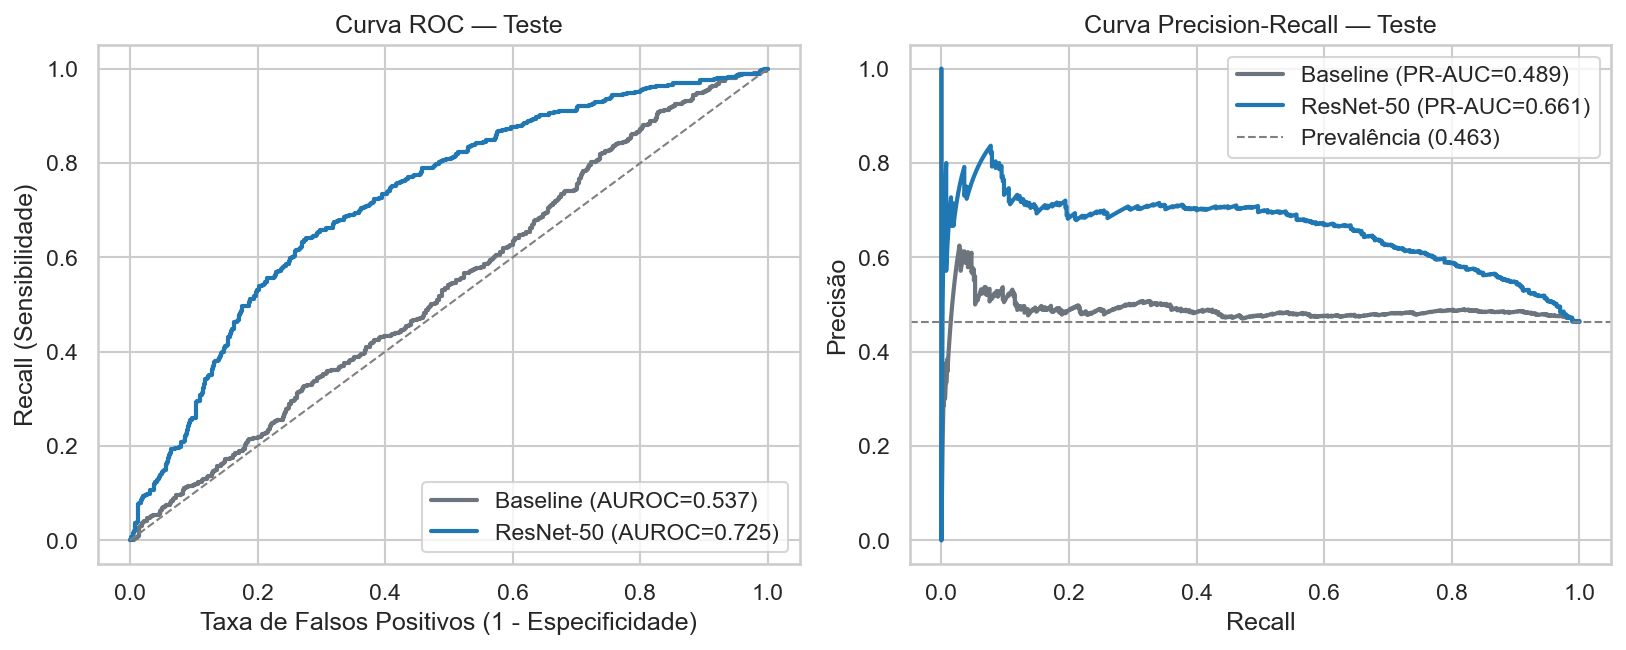
\includegraphics[width=.43\textwidth]{figuras/roc_pr.png}\hfill
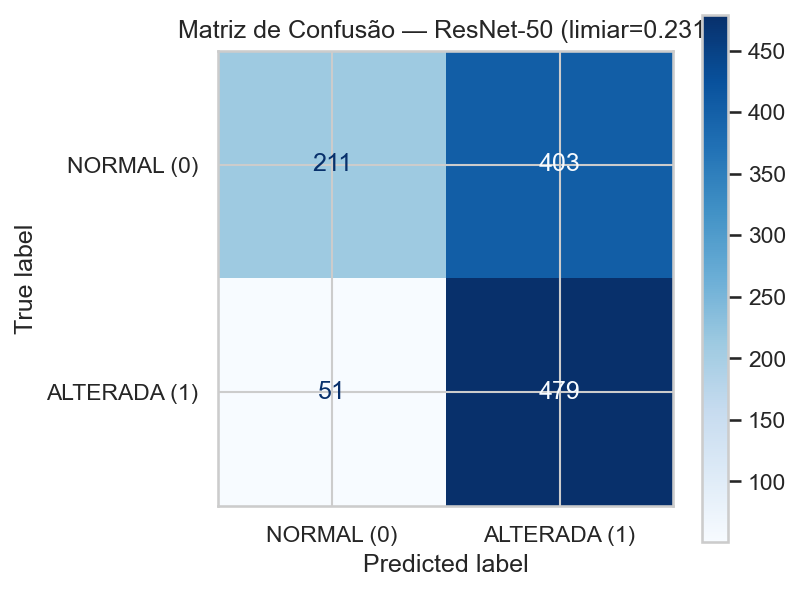
\includegraphics[width=.43\textwidth]{figuras/confusao_resnet50.png}
\caption{Curvas ROC/PR e matriz de confusão no teste. Fonte: \texttt{results/figures/}.}\label{fig:roc}
\end{figure}

Na camada de decisão sobre o teste, 44 imagens foram atribuídas a PRIORIDADE ALTA, 725 a PRIORIDADE MÉDIA, 188 a INDETERMINADO e 187 a ROTINA. Entre estas últimas, 34 tinham rótulo ALTERADA. A Tabela~\ref{tab:degradado} compara as versões originais e degradadas; os números vêm de \texttt{results/metrics/degraded\_by\_type.csv}. No conjunto pareado, o recall aumentou de 0,880 para 0,907, enquanto a precisão caiu de 0,564 para 0,511, o F1 de 0,688 para 0,654 e a balanced accuracy de 0,600 para 0,520. O aumento de recall ocorreu junto de mais falsos positivos, que passaram de 51 para 65. Não se deve ler o resultado como melhora geral.

\begin{table}[ht]
\centering\small
\caption{Desempenho no subconjunto pareado por degradação. Cada tipo tem 30 imagens. Fonte: \texttt{degraded\_by\_type.csv}.}\label{tab:degradado}
\begin{tabular}{lcrrrr}\toprule
Tipo & Versão & Recall & Precisão & F1 & Bal. acc.\\\midrule
Ruído & O/D & 0,800/1,000 & 0,480/0,500 & 0,600/0,667 & 0,467/0,500\\
Rotação & O/D & 0,867/0,933 & 0,650/0,500 & 0,743/0,651 & 0,700/0,500\\
Corte & O/D & 0,933/0,800 & 0,500/0,462 & 0,651/0,585 & 0,500/0,433\\
Baixo contraste & O/D & 0,867/0,800 & 0,619/0,632 & 0,722/0,706 & 0,667/0,667\\
Combinada & O/D & 0,933/1,000 & 0,609/0,500 & 0,737/0,667 & 0,667/0,500\\
Total & O/D & 0,880/0,907 & 0,564/0,511 & 0,688/0,654 & 0,600/0,520\\\bottomrule
\end{tabular}
\end{table}

A checagem de qualidade sinalizou 30 de 30 imagens de baixo contraste e 30 de 30 de corte, 13 de 30 combinadas e nenhuma de ruído ou rotação. O resultado de corte decorre da nitidez medida após o redimensionamento, e não prova que a regra identifica cortes de forma geral. No teste original, três das 150 imagens selecionadas foram sinalizadas. A figura de queda resume F1 e balanced accuracy por tipo.

\begin{figure}[ht]
\centering
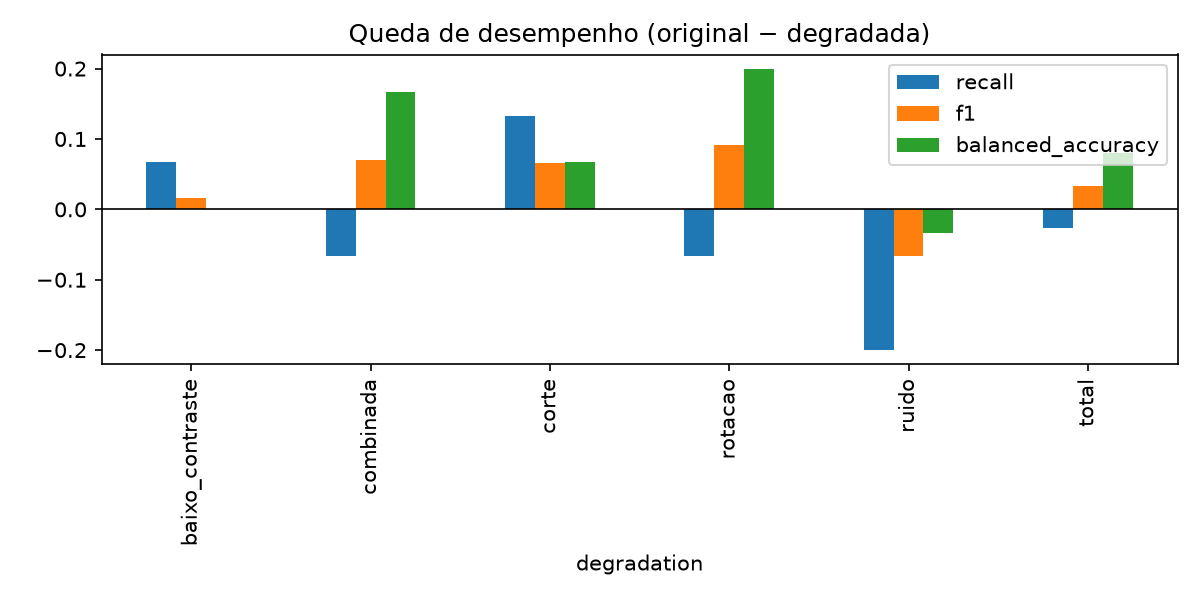
\includegraphics[width=.55\textwidth]{figuras/degradado_queda.png}
\caption{Diferença entre métricas das versões originais e degradadas; valores negativos indicam aumento na versão degradada. Fonte: \texttt{degradado\_queda.png}.}\label{fig:queda}
\end{figure}

A grade Grad-CAM da Figura~\ref{fig:cam} reúne 3 verdadeiros positivos, 3 falsos negativos, 3 falsos positivos e 3 verdadeiros negativos selecionados deterministicamente. Nos três falsos negativos, a ativação mais intensa aparece em bordas fora dos pulmões. Entre os verdadeiros positivos, dois apresentam foco predominante nos pulmões e um mistura área pulmonar e borda. A grade sem sobreposição, \texttt{results/figures/acertos\_erros.png}, mostra os exemplos com probabilidade, rótulo e saída da camada de decisão. As observações caso a caso estão em \texttt{results/gradcam\_casos.csv}. A atenção fora dos pulmões sugere possíveis atalhos visuais, mas o Grad-CAM não demonstra causalidade nem valida os rótulos clinicamente.

\begin{figure}[ht]
\centering
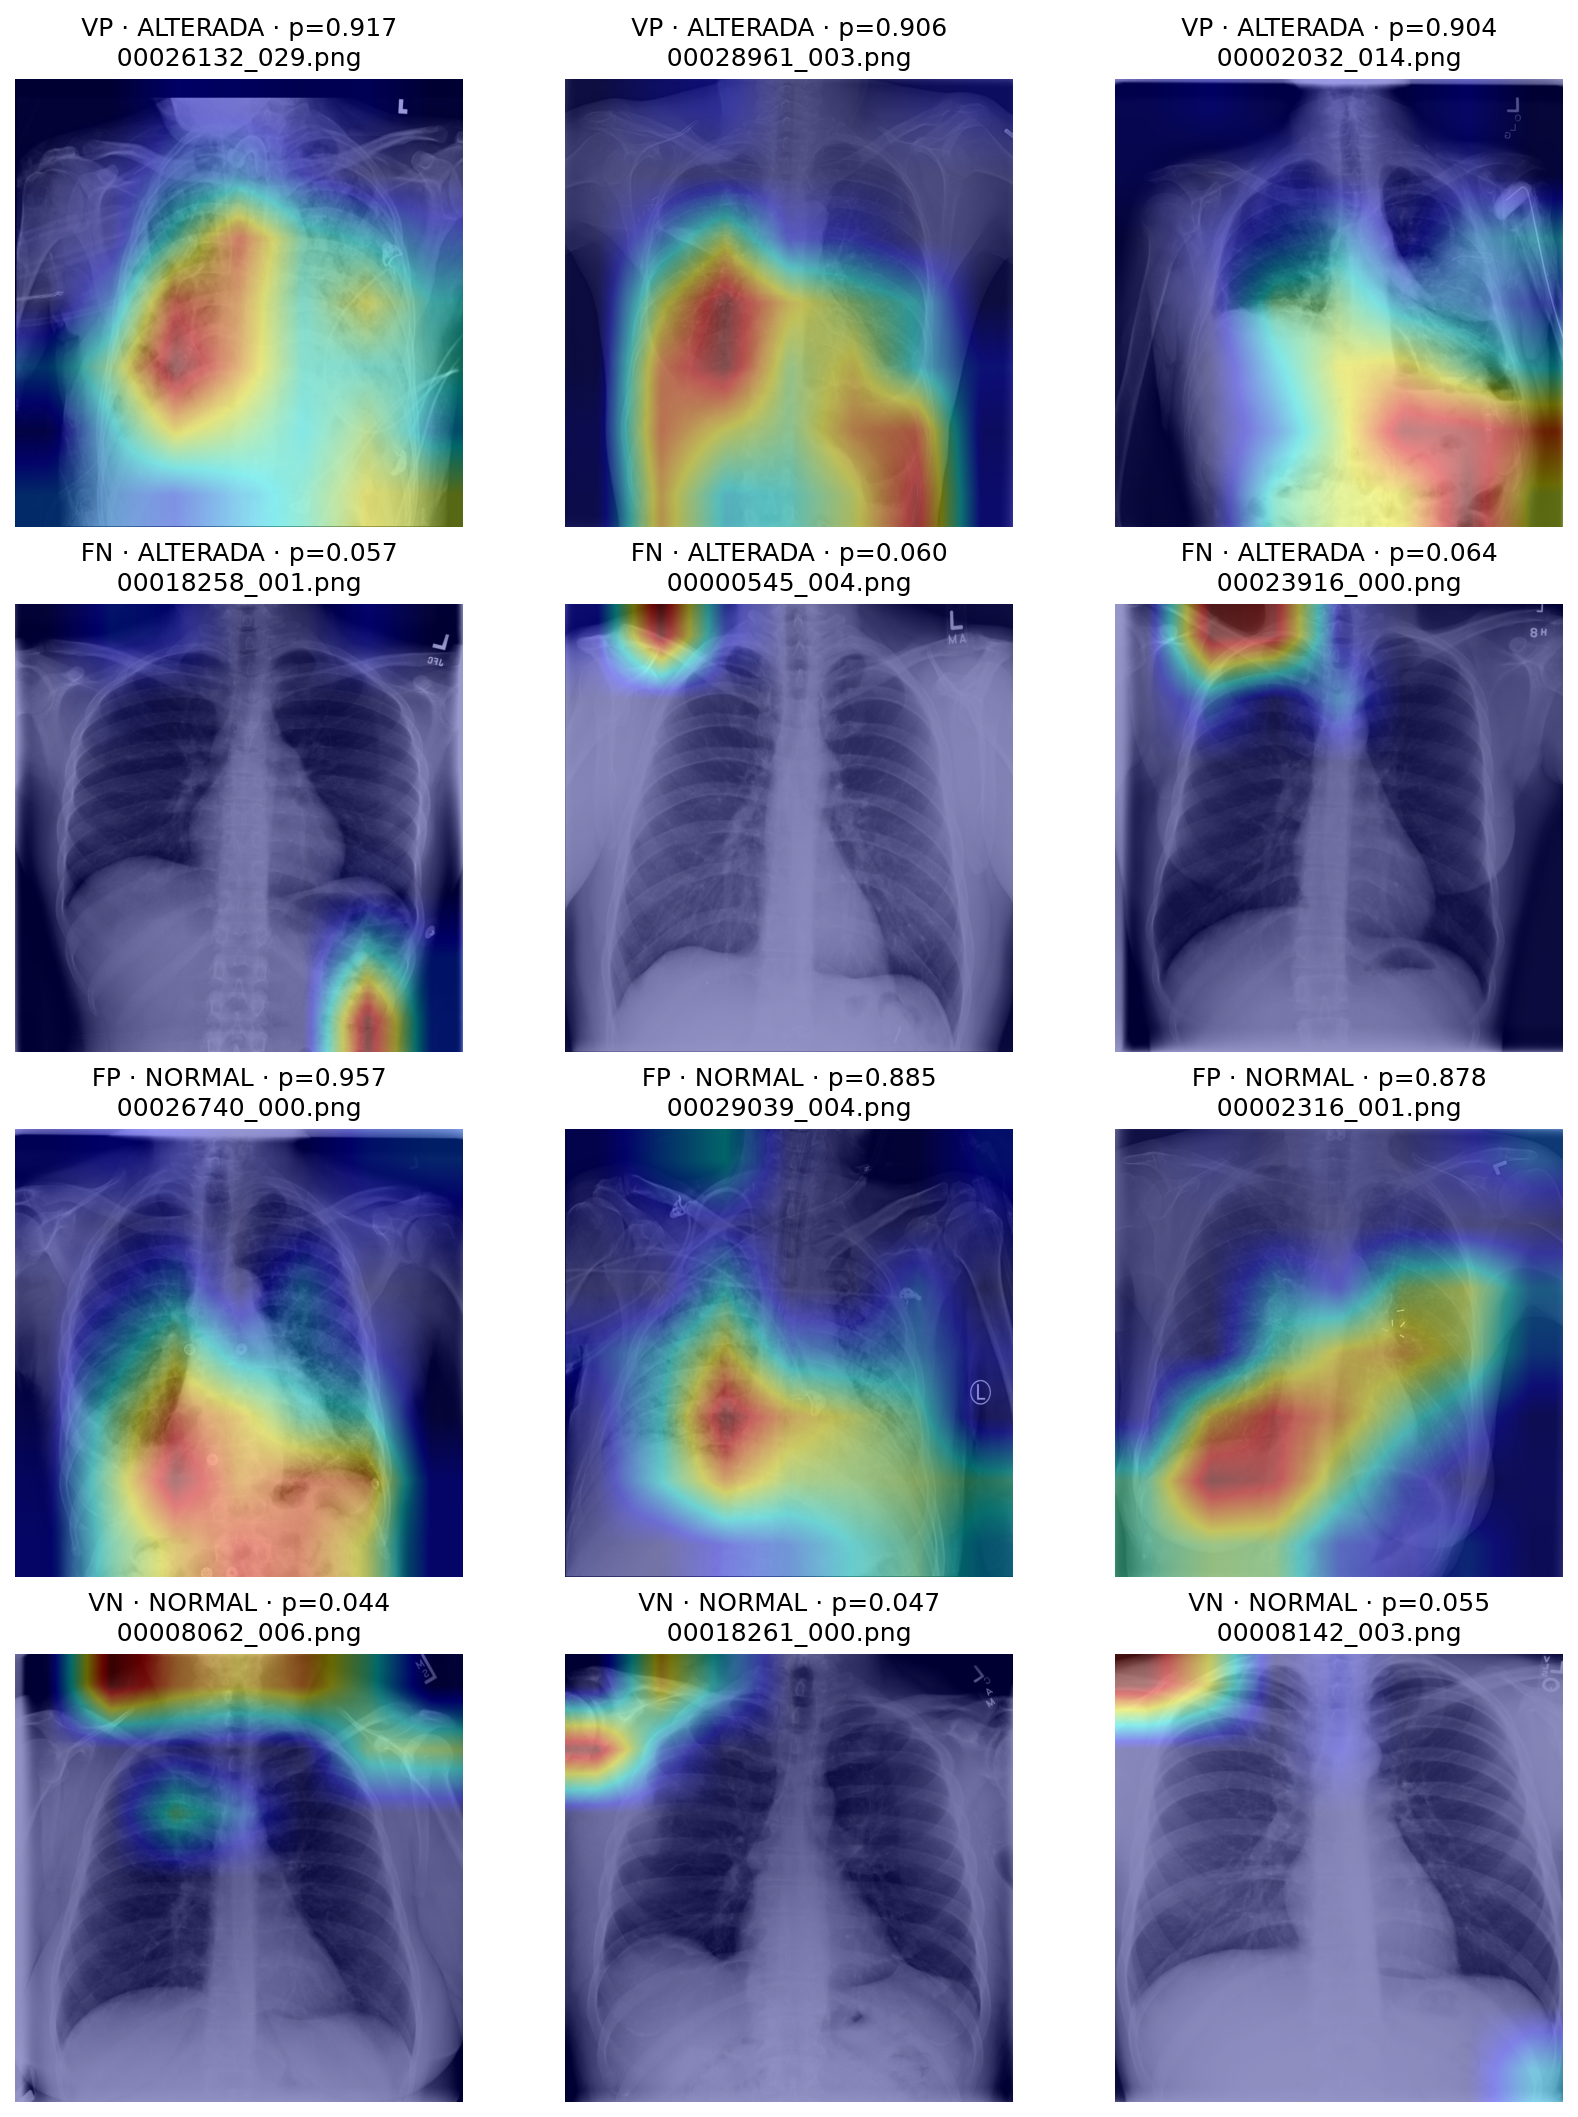
\includegraphics[width=.60\textwidth]{figuras/gradcam_teste.png}
\caption{Grad-CAM em 12 casos do teste, organizados por resultado da classificação. Fonte: \texttt{results/figures/gradcam\_teste.png}.}\label{fig:cam}
\end{figure}

\section{Conclusão}
A divisão por paciente e a comparação pareada permitiram medir desempenho e robustez com controle de vazamento entre treino e teste. O modelo alcançou recall elevado, à custa de muitos falsos positivos. Nas degradações, a balanced accuracy caiu, embora o recall tenha subido. A inspeção Grad-CAM encontrou ativações extra-pulmonares nos falsos negativos selecionados, motivando investigação de marcadores e bordas. Como próximos passos, são necessárias validação externa em outra instituição, calibração probabilística e detecção explícita de rotação e corte. O protótipo não deve orientar decisões clínicas sem validação adicional.

\bibliographystyle{sbc}
\bibliography{refs}
\end{document}


